\chapter{光照(Lighting)}
\begin{flushleft}
考虑图\ref{fig:8-1}。 在左边我们有一个没有照明的球体,在右边,我们有一个点亮的球体。 正如你所看到的,左边的球体看起来很平坦——也许它根本不是一个球体,而只是一个2D圆圈! 另一方面,右侧的球体确实看起来是3D——照明和阴影有助于我们对物体的固体形状和体积的感知。 事实上,我们对世界的视觉感知取决于光线及其与材料的相互作用,因此,产生逼真场景的大部分问题都与物理上精确的照明模型有关。
\end{flushleft}

\begin{figure}[h]
    \label{fig:8-1}
    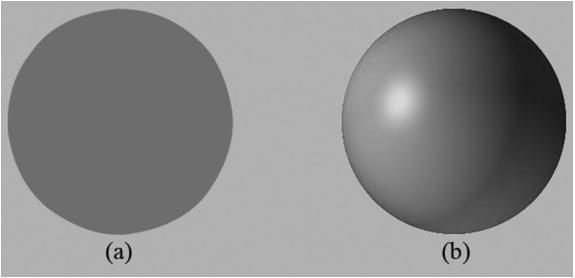
\includegraphics[width=\textwidth]{8-1}
    \centering
    \caption{(a)未点亮的球体看起来是2D。(b)点亮的球体看起来是3D。}
\end{figure}

\begin{flushleft}
当然,一般来说,模型越准确,计算成本越高; 因此,必须在现实主义和速度之间达成平衡。 例如,用于电影的3D特殊FX场景可以比游戏更复杂并且使用非常逼真的照明模型,因为电影的帧是预渲染的,因此它们可以花费数小时或数天来处理帧。 另一方面,游戏是实时应用程序,因此,帧需要以每秒至少30帧的速率绘制。\\
请注意,本书中解释和实现的照明模型很大程度上基于[Möller08]中描述的模型。\\
~\\
{\large Objectives:}
\begin{itemize}
    \item 了解灯光和材料之间的相互作用
    \item 了解局部照明和全局照明之间的差异
    \item 了解我们如何在数学上描述表面上的一个点“朝向”的方向,以便我们可以确定入射光照射到表面的角度
    \item 学习如何正确转换法向量
    \item 能够区分环境光,漫反射光和镜面光
    \item 了解如何实现定向灯,指示灯和聚光灯
    \item 通过控制衰减参数来了解如何根据深度改变光强度
\end{itemize}
\end{flushleft}

%------- 8.1 ---------------
\section{光与材质的相互作用(Light And Meterial Interaction)}
\begin{flushleft}
使用灯光时,我们不再直接指定顶点颜色; 相反,我们指定材质和灯光,然后应用光照方程式,根据光/材料相互作用计算我们的顶点颜色。 这样可以使对象更加逼真地着色(再次比较图\ref{fig:8-1}a和\ref{fig:8-1}b)。\\
可以将材质视为确定光如何与对象表面相互作用的属性。 比如表面反射和吸收的光的颜色,表面下材料的折射率,表面的光滑程度以及表面的透明度。 通过指定材质属性,我们可以模拟不同类型的真实世界表面,如木材,石材,玻璃,金属和水。\\
在我们的模型中,光源可以发出各种强度的红色,绿色和蓝色光; 通过这种方式,我们可以模拟许多浅色。 当光从光源向外传播并与物体碰撞时,一些光可能被吸收而一些光可能被反射(对于透明物体,例如玻璃,一些光线穿过介质,但我们不考虑这里的透明度)。 反射光现在沿着其新的路径行进并且可能撞击其他物体,其中一些光再次被吸收和反射。 在完全吸收之前,光线可能会撞击许多物体。 据推测,一些光线最终会进入眼睛(见图\ref{fig:8-2})并撞击视网膜上的光受体细胞(称为视锥细胞和视杆细胞)。\\
\end{flushleft}

\begin{figure}[h]
    \label{fig:8-2}
    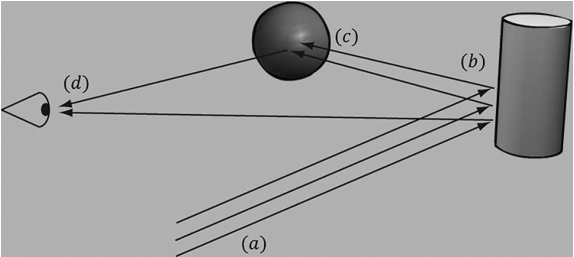
\includegraphics[width=\textwidth]{8-2}
    \centering
    \caption{(a)入射白光的通量。(b)光线照射到圆柱体上,一些光线被吸收,其他光线散射到眼睛和球体上。(c)从圆筒向球体反射的光被再次吸收或反射并进入眼睛。(d)眼睛接收入射光,确定眼睛看到的是什么。}
\end{figure}

\begin{flushleft}
根据三色理论(见[Santrock03]),视网膜含有三种光受体,每种受体对红光,绿光和蓝光敏感(有一些重叠)。 入射的RGB光根据光的强度对其相应的光接收器产生不同强度的刺激。 当光受体受到刺激(或不被刺激)时,神经冲动沿着视神经向大脑发送,大脑基于光受体的刺激在大脑中产生图像。 (当然,如果你闭上/遮住眼睛,受体细胞就不会受到任何刺激,大脑会将其记录为黑色。)\\

例如,再次考虑图\ref{fig:8-2}。假设圆柱体的材料反射75%的红光,75%的绿光,并吸收其余部分,球体反射25%的红光并吸收其余部分。还假设从光源发射纯白光。当光线照射到圆柱体上时,所有的蓝光都被吸收,只有75%的红光和绿光被反射(即,中高强度的黄色)。然后这种光被散射——其中一些光进入眼睛,一些光线向球体传播。进入眼睛的部分主要刺激红色和绿色锥形细胞达到半高度;因此,观察者将圆柱视为半亮的黄色阴影。现在,其他光线向球体射出并撞击它。球体反射25%的红光并吸收其余部分;因此,稀释的入射红光(中高强度红色)被进一步稀释并反射,并且所有进入的绿光被吸收。这剩余的红光然后进入眼睛并较低程度地刺激红锥细胞。因此,观察者将球体视为深红色。\\
我们(和大多数实时应用)在本书中采用的照明模型称为局部照明模型。 使用局部模型,每个对象独立于另一个对象被点亮,并且在光照过程中仅考虑从光源直接发射的光(即,从其他场景对象反弹以击中当前被点亮的对象的光是忽略的)。 图\ref{fig:8-3}显示了该模型的结果。
\end{flushleft}

\begin{figure}[h]
    \label{fig:8-3}
    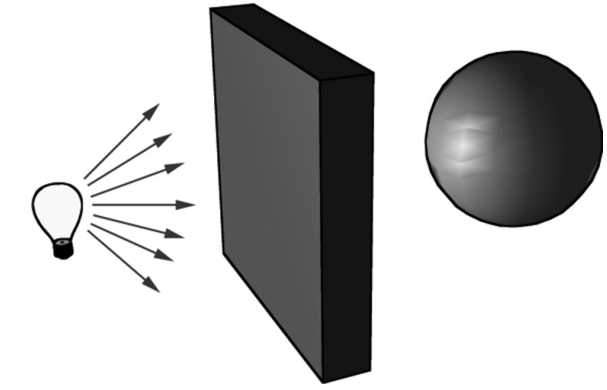
\includegraphics[width=\textwidth]{8-3}
    \centering
    \caption{在物理上,墙壁阻挡了灯泡发出的光线,并且球体位于墙壁的阴影中。 然而,在局部照明模型中,球体被照亮,好像墙壁不存在一样。}
\end{figure}

\begin{flushleft}
另一方面,全局照明通过不仅考虑从光源直接发射的光而且还考虑从场景中的其他物体反弹的间接光来模拟光物体。 这些被称为全局照明模型,因为它们在照亮对象时会考虑全局场景中的所有内容。 对于实时游戏而言,全局照明模型通常过于昂贵(但非常接近于生成逼真的场景)。 寻找近似全局照明的实时方法是一个正在进行研究的领域; 例如,参见\href{http://on-demand.gputechconf.com/gtc/2014/presentations/S4552-rt-voxel-based-global-illumination-gpus.pdf}{\textcolor{linkColor}{voxel global illumination}}。 其他流行的方法是预先计算静态对象(例如,墙壁,雕像)的间接照明,然后使用该结果来近似动态对象的间接照明(例如,移动游戏角色)。\\
\end{flushleft}

%------- 8.2 ---------------
\section{法向量(Normal Vectors)}
\begin{flushleft}
面法线(face normal)是描述多边形正面朝向的单位矢量(即,它与多边形上的所有点正交); 见图\ref{fig:8-4}a。 表面法线是与表面上的点的切平面正交的单位矢量; 见图\ref{fig:8-4}b。 观察表面法线确定表面上的点“朝向”的方向。\\
\end{flushleft}

\begin{figure}[h]
    \label{fig:8-4}
    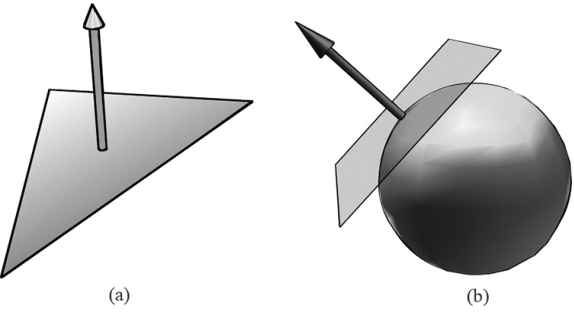
\includegraphics[width=\textwidth]{8-4}
    \centering
    \caption{(a)面部法线与面部上的所有点正交。 (b)表面法线是与表面上的点的切平面正交的矢量。}
\end{figure}

\begin{figure}[h]
    \label{fig:8-5}
    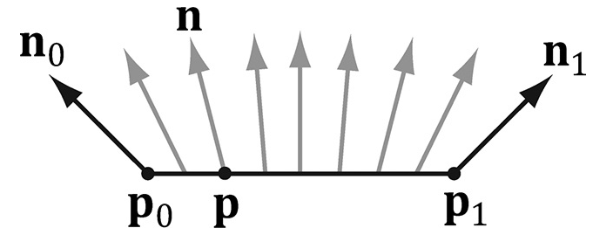
\includegraphics[width=\textwidth]{8-5}
    \centering
    \caption{顶点法线$n_{0}$和$n_{1}$在段顶点$p_{0}$和$p_{1}$处定义。 通过在顶点法线之间进行线性插值(加权平均),找到线段内部的点$p$的法向量$n$; 也就是说,$p=p_{0}+t(p_{1}-p_{0})$,其中$t$代表$p_{0}p$与$p_{0}p_{1}$的比例,则$p$的法线$n=n_{0} + t(n_{1}-n_{0})$。尽管为了简单起见我们在线段上表现了正常插值,但这个想法可以直观地应用在3D三角形上。}
\end{figure}

\begin{flushleft}
对于光照计算,我们需要在三角形网格表面上的每个点处的曲面法线,以便我们可以确定光线照射到网格曲面上的点的角度。 为了获得曲面法线,我们仅在顶点处指定曲面法线(所谓的顶点法线)。 然后,为了在三角形网格的表面上的每个点处获得近似的表面法线,这些顶点法线将在光栅化期间在三角形上插值(回忆5.10.3节并参见图\ref{fig:8-5})。\\
~\\
NOTICE: 对每个像素的法线和光照计算进行插值称为像素照明或phong照明。 一种较便宜但不太精确的方法是每个顶点进行照明计算。 然后,从顶点着色器输出每顶点光照计算的结果,并在三角形的像素上进行插值。 将像素着色器移动到顶点着色器的计算是质量方面的常见性能优化,有时视觉差异非常小,使得这种优化非常有吸引力。\\
\end{flushleft}

%------- 8.2.1 ---------------
\subsection{计算法向量(Computing Normal Vectors)}
\begin{flushleft}
为了找到三角形$p_{0}$,$p_{1}$,$p_{2}$的面法线,我们首先计算位于三角形边缘的两个向量:\\
\end{flushleft}

\begin{align*}
u=p_{1}-p_{0}\\
v=p_{2}-p_{0}
\end{align*}

\begin{flushleft}
然后,其面法向量为:\\
\end{flushleft}

\begin{align*}
n=\frac{u\times v}{||u\times v||}
\end{align*}

\begin{flushleft}
下面是一个函数,用于计算三角形三个顶点的三角形正面(5.10.2节)的面法线。\\
\end{flushleft}

\begin{lstlisting}
XMVECTOR ComputeNormal(FXMVECTOR p0, FXMVECTOR p1, FXMVECTOR p2)
{
    XMVECTOR u = p1 - p0;
    XMVECTOR v = p2 - p0;
    return XMVector3Normalize(XMVector3Cross(u,v));
}
\end{lstlisting}

\begin{figure}[h]
    \label{fig:8-6}
    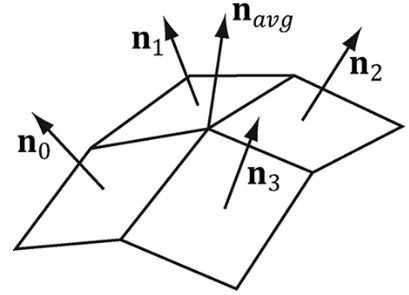
\includegraphics[width=\textwidth]{8-6}
    \centering
    \caption{中间顶点由相邻的四个多边形共享,因此我们通过平均四个多边形面法线来近似中间顶点法线。}
\end{figure}

\begin{flushleft}
对于可微分的表面,我们可以使用微积分来找到曲面上的法线。 不幸的是,三角形网格不可区分。 通常应用于三角形网格的技术称为顶点法线平均(vetex normal averaging)。 网格中的顶点法线$n$或任意顶点$v$是通过平均共享顶点$v$的网格中每个多边形的面法线来找到的。例如,在图\ref{fig:8-6}中,网格中的四个多边形因此共享顶点$v$, $v$的顶点法线由下式给出:\\
\end{flushleft}

\begin{align*}
n_{avg}=\frac{n_{0}+n_{1}+n_{2}+n_{3}}{||n_{0}+n_{1}+n_{2}+n_{3}||}
\end{align*}

\begin{flushleft}
在上面的例子中,我们不需要除以4,就像我们在典型的平均值中那样,因为我们将结果标准化。 还要注意,可以构建更复杂的平均方案; 例如,可以使用加权平均值,其中权重由多边形的面积确定(例如,具有较大区域的多边形比具有较小区域的多边形具有更多权重)。\\
以下伪代码显示了如何在给定三角形网格的顶点和索引列表的情况下实现此平均:\\
\end{flushleft}

\begin{lstlisting}
// Input:
// 1. An array of vertices (mVertices). Each vertex has a
// position component (pos) and a normal component (normal).
// 2. An array of indices (mIndices).
// For each triangle in the mesh:
for(UINT i = 0; i < mNumTriangles; ++i)
{
    // indices of the ith triangle
    UINT i0 = mIndices[i*3+0];
    UINT i1 = mIndices[i*3+1];
    UINT i2 = mIndices[i*3+2];

    // vertices of ith triangle
    Vertex v0 = mVertices[i0];
    Vertex v1 = mVertices[i1];
    Vertex v2 = mVertices[i2];

    // compute face normal
    Vector3 e0 = v1.pos - v0.pos;
    Vector3 e1 = v2.pos - v0.pos;
    Vector3 faceNormal = Cross(e0, e1);

    // This triangle shares the following three vertices,
    // so add this face normal into the average of these
    // vertex normals.
    mVertices[i0].normal += faceNormal;
    mVertices[i1].normal += faceNormal;
    mVertices[i2].normal += faceNormal;
}
// For each vertex v, we have summed the face normals of all
// the triangles that share v, so now we just need to normalize.
for(UINT i = 0; i < mNumVertices; ++i)
    mVertices[i].normal = Normalize(&mVertices[i].normal));
\end{lstlisting}

%------- 8.2.2 ---------------
\subsection{转换法向量(Transforming Normal Vectors)}
\begin{flushleft}
考虑图\ref{fig:8-7}a,其中我们具有与法向量$n$正交的切向量$u=v_{1}-v_{0}$。 如果我们应用非均匀缩放变换$A$,我们从图\ref{fig:8-7}b中看到,变换的切向量$uA=v_{1}A-v_{0}A$不与变换的法向量$nA$保持正交。
\end{flushleft}

\begin{figure}
\label{fig:8-7}
\begin{subfigure}{1\textwidth}
  \centering
  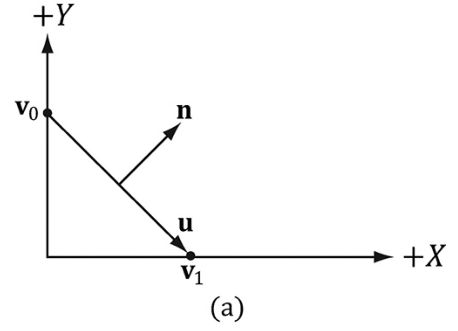
\includegraphics[width=1\linewidth]{8-7-a}
\end{subfigure}
\begin{subfigure}{1\textwidth}
  \centering
  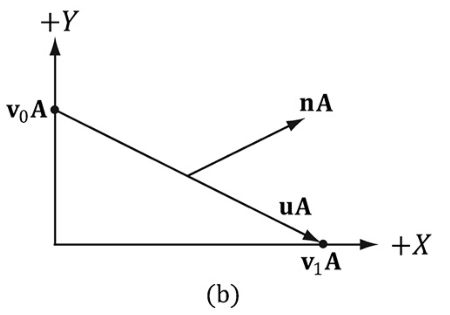
\includegraphics[width=1\linewidth]{8-7-b}
\end{subfigure}
\begin{subfigure}{1\textwidth}
  \centering
  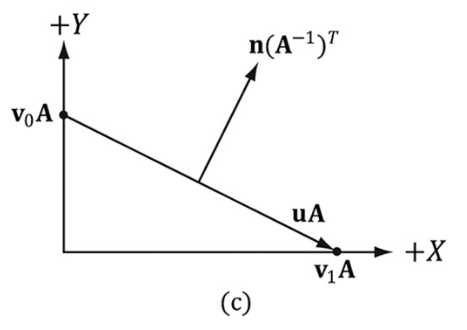
\includegraphics[width=1\linewidth]{8-7-c}
\end{subfigure}
\caption{(a)转变前的表面法线。(b)在x轴上缩放2个单位后,法线不再与表面正交。 (c)通过缩放变换的逆转置正确地变换的表面法线。}
\end{figure}

\begin{flushleft}
所以我们的问题是:给定转换矩阵$A$转换点和向量(非正态),我们想找到一个转换矩阵$B$,使得转换的切线向量与转换的法向量正交(即 $uA\cdot nB = 0$)。 要做到这一点,首先从我们知道的东西开始:我们知道法向量$n$与切向量$u$正交:\\
\end{flushleft}

\begin{tabular}{|p{5em}|p{35em}|} 
\hline
$u\cdot n=0$ & 切线向量与法向量正交\\ 
\hline
$un^{T}=0$ & 将点积重写为矩阵乘法\\ 
\hline
$u(AA^{-1})n^{T}=0$ & 插入单位矩阵$I=AA^{-1}$\\
\hline 
$(uA)(A^{-1}n^{T})=0$ & 矩阵乘法结合律\\
\hline 
$(uA)(((A^{-1}n^{T})^{T})^{T})=0$ & 矩阵转置性质:$(A^{T})^{T}=A$\\
\hline 
$(uA)((n(A^{-1})^{T})^{T})=0$ & 矩阵转置性质:$(AB^{T})^{T}=B^{T}A^{T}$\\
\hline 
$uA\cdot n(A^{-1})^{T}=0$ & 将矩阵乘法重写为点积\\ 
\hline
$uA\cdot nB=0$ & 经B转换的法向量与经A转换的法向量正交\\ 
\hline
\end{tabular}

\begin{flushleft}
因此,$B=(A^{-1})^{T}$(A的逆转置)在转换法向量时起作用,使得它们垂直于其相关的变换切线向量$uA$。\\

注意,如果矩阵是正交的(正交矩阵$(A^{T}=A^{-1})$),则$B=(A^{-1})^{T}=(A^{T})^{T}=A$; 也就是说,我们不需要计算逆转置,因为A在这种情况下完成了工作。 总之,当通过非均匀或剪切变换转换法向量时,请使用逆转置。\\
我们在 MathHelper.h 中实现了一个辅助函数来计算逆转换:\\
\end{flushleft}

\begin{lstlisting}
static XMMATRIX InverseTranspose(CXMMATRIX M)
{
    XMMATRIX A = M;
    A.r[3] = XMVectorSet(0.0f, 0.0f, 0.0f, 1.0f);
    XMVECTOR det = XMMatrixDeterminant(A);
    return XMMatrixTranspose(XMMatrixInverse(&det, A));
}
\end{lstlisting}

\begin{flushleft}
我们清除矩阵中的任何平移转换,因为我们使用逆转置来转换向量,并且转换仅适用于点。 但是,根据 3.2.1 节,我们知道为向量设置$w=0$(使用齐次坐标)可以防止向量被平移变换修改。 因此,我们不应该将矩阵中的平移归零。 问题是如果我们想要连接逆转置和不包含非均匀缩放的另一个矩阵,比如视图矩阵$(A^{-1})^{T}V$,$(A^{-1})^{T}$的第四列中的转置平移"泄漏"(leaks)到矩阵乘法运算导致错误。因此,我们将平移归零以作为预防措施以避免此错误。 正确的方法是通过以下方式转换法线:$((AV)^{-1})^{T}$。 下面是缩放和平移矩阵的示例,以及第四列不是$[0,0,0,1]^{T}$的逆转置看起来是什么样的:\\
\end{flushleft}

\begin{align*}
A&=
\begin{bmatrix}
1 & 0 & 0 & 0\\
0 & 0.5 & 0 & 0\\
0 & 0 & 0.5 & 0\\
1 & 1 & 1 & 1
\end{bmatrix}\\
(A^{-1})^{T}&=
\begin{bmatrix}
1 & 0 & 0 & -1\\
0 & 2 & 0 & -2\\
0 & 0 & 2 & -2\\
0 & 0 & 0 & 1
\end{bmatrix}
\end{align*}

\begin{flushleft}
NOTICE: 即使使用逆转置变换,法向量也可能失去单位长度; 因此,它们可能需要在转换后重新规范化。
\end{flushleft}

%------- 8.3 ---------------
\section{照明中的重要向量(Important Vectors In Lighting)}
\begin{flushleft}
在本节中,我们总结了一些与照明有关的重要向量。参考图\ref{fig:8-8},$E$是眼睛位置,我们正在考虑眼睛沿着由单位向量$v$定义的位置线看到的点$p$。在点$p$ 处,表面具有法向量$n$,并且该点被一个入射方向$I$的光线击中。光向量$L$是朝向撞击表面点的光线的相反方向的单位矢量。虽然使用光传播方向可能更直观,但对于光照计算,我们使用光向量$L$;特别地,为了计算朗伯余弦定律(Lambert’s Cosine Law),向量$L$用于计算$L\cdot n=cos\Theta_{i}$,其中$\Theta_{i}$是$L$和$n$之间的角度。反射向量$r$是关于表面法线$n$的入射光向量的反射。视图向量(或眼睛向量)$v$=标准化$(E-p)$是从表面点$p$到眼点$E$的单位向量,其定义从眼睛到被观察表面上的点的位置线。有时我们需要使用矢量$-v$,它是从眼睛到表面上我们正在计算光照的点的单位向量。\\
\end{flushleft}

\begin{figure}[h]
    \label{fig:8-8}
    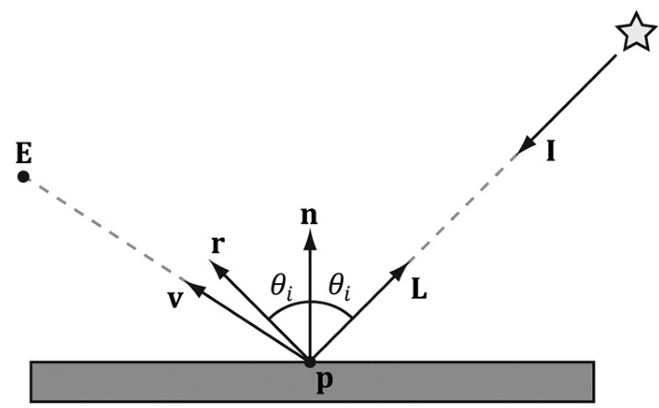
\includegraphics[width=\textwidth]{8-8}
    \centering
    \caption{光照计算中涉及到的重要向量}
\end{figure}

\begin{flushleft}
反射向量由下式给出:$r=I-2(n\cdot I)n$; 见图\ref{fig:8-9}。 (假设$n$是单位向量。)但是,我们实际上可以使用HLSL内部反射函数在着色器程序中为我们计算$r$。
\end{flushleft}

\begin{figure}[h]
    \label{fig:8-9}
    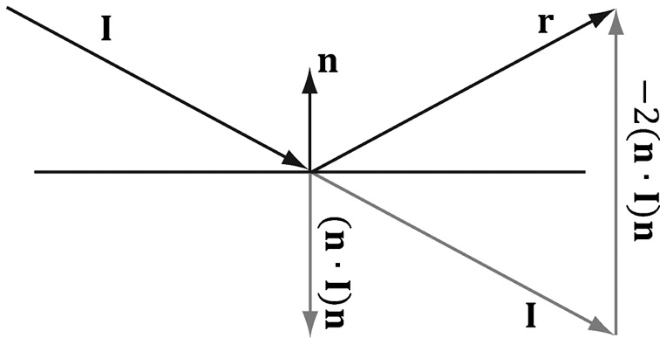
\includegraphics[width=\textwidth]{8-9}
    \centering
    \caption{反射几何}
\end{figure}

%------- 8.4 ---------------
\section{朗伯余弦定律(Lambert’s Cosine Law)}







